% Author   : Alain Matthes
% Encoding : UTF8
% Engine   : PDFLaTeX
% from http://www.fauskes.net/media/code/blend2sketch/img/boxann.png
\documentclass[]{article}
\usepackage[utf8]{inputenc} 
\usepackage{fullpage}
\usepackage{fourier}
\usepackage{tikz}
\usetikzlibrary{calc,3d}

\begin{document}
\thispagestyle{empty} 

\begin{center}
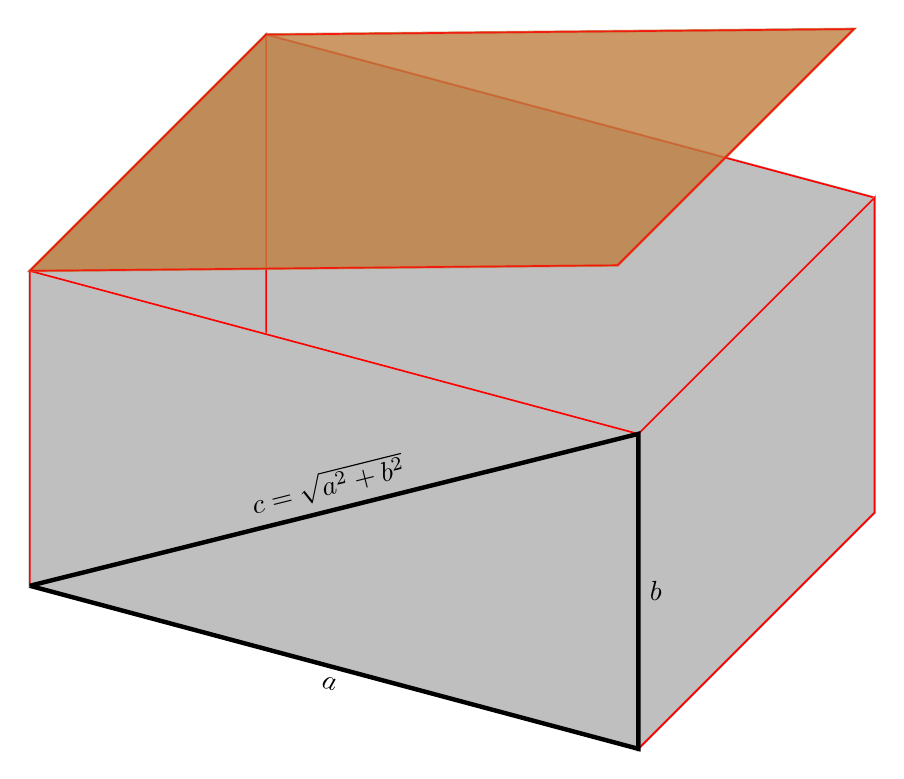
\begin{tikzpicture}[x     = {(-0.5cm,-0.5cm)},
                    y     = {(0.9659cm,-0.25882cm)},
                    z     = {(0cm,1cm)},
                    scale = 2,
                    color = {lightgray}]
% style of faces
\tikzset{facestyle/.style={fill,draw=lightgray,double=red,very thin}}
% face "back" 
\begin{scope}[canvas is zy plane at x=0]
  \path[facestyle] (0,0) rectangle (2,4);
\end{scope}
% face  "left"
\begin{scope}[canvas is zx plane at y=0]
  \path[facestyle] (0,0) rectangle (2,3);
\end{scope}
% face "front"
\begin{scope}[canvas is zy plane at x=3]
  \path[facestyle] (0,0) rectangle (2,4);
\end{scope}
% face  "right"
\begin{scope}[canvas is zx plane at y=4]
  \path[facestyle] (0,0) rectangle (2,3);
\end{scope}
% face "up" 
\draw[fill=brown,draw=brown,double=red,opacity=.8,very thin]
 (0,0,2) -- 
 (3,0,2) --
 (3,{4*cos(15)},{4*sin(15)+2}) --
 (0,{4*cos(15)},{4*sin(15)+2}) --cycle ;
% labels
\draw[ultra thick,black]
     (3,0,0) -- node [sloped,below] {$a$}    
     (3,4,0) -- node [right]        {$b $}
     (3,4,2) -- node [sloped,above] {$c=\sqrt{a^2+b^2}$} 
     (3,0,0);
\end{tikzpicture}
\end{center}
\end{document}
